
\documentclass[]{article}
\voffset=-1.5cm
\oddsidemargin=0.0cm
\textwidth = 480pt

% http://www.strath.ac.uk/aer/materials/5furtherquantitativeresearchdesignandanalysis/unit6/whatislogisticregression/

% http://www.medcalc.org/manual/logistic_regression.php


\usepackage{amsmath}
\usepackage{graphicx}
\usepackage{amssymb}
\usepackage{framed}
\usepackage{multicol}
%\usepackage[paperwidth=21cm, paperheight=29.8cm]{geometry}
%\usepackage[angle=0,scale=1,color=black,hshift=-0.4cm,vshift=15cm]{background}
%\usepackage{multirow}
\usepackage{enumerate}






\begin{document}
\section{Wilcoxon Signed-Rank Test using SPSS Statistics}

\subsection{Introduction}
The Wilcoxon signed-rank test is the nonparametric test equivalent to the dependent t-test. As the Wilcoxon signed-rank test does not assume normality in the data, it can be used when this assumption has been violated and the use of the dependent t-test is inappropriate. It is used to compare two sets of scores that come from the same participants. This can occur when we wish to investigate any change in scores from one time point to another, or when individuals are subjected to more than one condition.

For example, you could use a Wilcoxon signed-rank test to understand whether there was a difference in smokers' daily cigarette consumption before and after a 6 week hypnotherapy programme (i.e., your dependent variable would be "daily cigarette consumption", and your two related groups would be the cigarette consumption values "before" and "after" the hypnotherapy programme). You could also use a Wilcoxon signed-rank test to understand whether there was a difference in reaction times under two different lighting conditions (i.e., your dependent variable would be "reaction time", measured in milliseconds, and your two related groups would be reaction times in a room using "blue light" versus "red light").

This "quick start" guide shows you how to carry out a Wilcoxon signed-rank test using SPSS Statistics, as well as interpret and report the results from this test. However, before we introduce you to this procedure, you need to understand the different assumptions that your data must meet in order for a Wilcoxon signed-rank test to give you a valid result. We discuss these assumptions next.

\subsection{Assumptions}
When you choose to analyse your data using a Wilcoxon signed-rank test, part of the process involves checking to make sure that the data you want to analyse can actually be analysed using a Wilcoxon signed-rank test. You need to do this because it is only appropriate to use a Wilcoxon signed-rank test if your data "passes" three assumptions that are required for a Wilcoxon signed-rank test to give you a valid result. The first two assumptions relate to your study design and the types of variables you measured. The third assumption reflects the nature of your data and is the one assumption you test using SPSS Statistics. These three assumptions as briefly explained below:
\begin{description}
\item[Assumption 1:] Your dependent variable should be measured at the ordinal or continuous level. Examples of ordinal variables include Likert scales (e.g., a 7-point scale from "strongly agree" through to "strongly disagree"), amongst other ways of ranking categories (e.g., a 5-point scale explaining how much a customer liked a product, ranging from "Not very much" to "Yes, a lot"). 
\begin{itemize}
\item Examples of continuous variables (i.e., interval or ratio variables) include revision time (measured in hours), intelligence (measured using IQ score), exam performance (measured from 0 to 100), weight (measured in kg), and so forth. 
\end{itemize}
\item[Assumption 2:] Your independent variable should consist of two categorical, "related groups" or "matched pairs". "Related groups" indicates that the same subjects are present in both groups. The reason that it is possible to have the same subjects in each group is because each subject has been measured on two occasions on the same dependent variable. For example, you might have measured 10 individuals' performance in a spelling test (the dependent variable) before and after they underwent a new form of computerized teaching method to improve spelling. 
\begin{itemize}
	\item You would like to know if the computer training improved their spelling performance. The first related group consists of the subjects at the beginning (prior to) the computerized spelling training and the second related group consists of the same subjects, but now at the end of the computerized training. 
	\item The Wilcoxon signed-rank test can also be used to compare different subjects within a "matched-pairs" study design, but this does not happen very often. 
\end{itemize}


%%Nonetheless, to learn more about the different study designs you use with a Wilcoxon signed-rank test, see our enhanced Wilcoxon signed-rank test guide.

\item[Assumption 3:] The distribution of the differences between the two related groups (i.e., the distribution of differences between the scores of both groups of the independent variable; for example, the reaction time in a room with "blue lighting" and a room with "red lighting") needs to be symmetrical in shape. 
\begin{itemize}
	\item If the distribution of differences is symmetrically shaped, you can analyse your study using the Wilcoxon signed-rank test. In practice, checking for this assumption just adds a little bit more time to your analysis, requiring you to click a few more buttons in SPSS Statistics when performing your analysis, as well as think a little bit more about your data, but it is not a difficult task. However, do not be surprised if, when analysing your own data using SPSS Statistics, this assumption is violated (i.e., is not met). \item This is not uncommon when working with real-world data rather than textbook examples, which often only show you how to carry out a Wilcoxon signed-rank test when everything goes well! 
	\item However, even when your data fails this assumption, there is often a solution to overcome this, such as transforming your data to achieve a symmetrically-shaped distribution of differences (not a preferred option) or running a sign test instead of the Wilcoxon signed-rank test.
\end{itemize} 

If you are unsure of the procedures in SPSS Statistics to test this assumption or how to interpret the SPSS Statistics output, we show you how in our enhanced Wilcoxon signed-rank test guide, which you can access by subscribing to the site here.
In the section, Test Procedure in SPSS Statistics, we illustrate the SPSS Statistics procedure to perform a Wilcoxon signed-rank test. First, we introduce the example that is used in this "quick start" guide.
\end{description}
%=======================================================%
\subsection{Example}
A pain researcher is interested in finding methods to reduce lower back pain in individuals without having to use drugs. The researcher thinks that having acupuncture in the lower back might reduce back pain. To investigate this, the researcher recruits 25 participants to their study. At the beginning of the study, the researcher asks the participants to rate their back pain on a scale of 1 to 10, with 10 indicating the greatest level of pain. After 4 weeks of twice weekly acupuncture, the participants are asked again to indicate their level of back pain on a scale of 1 to 10, with 10 indicating the greatest level of pain. The researcher wishes to understand whether the participants' pain levels changed after they had undergone the acupuncture, so a Wilcoxon signed-rank test is run.



%==============================================================%
\subsection{Test Procedure in SPSS Statistics}
The six steps below show you how to analyse your data using a Wilcoxon signed-rank test in SPSS Statistics. At the end of these six steps, we show you how to interpret the results from this test.

Click Analyze > Nonparametric Tests > Legacy Dialogs > 2 Related Samples... on the top menu, as shown below:

Note: We show you the legacy procedure in SPSS Statistics to run the Wilcoxon signed-rank test below since this can be used with older versions of SPSS Statistics (17 and below), as well as more recent versions (version 18 and above). However, you can also run the Wilcoxon signed-rank test using the new procedure in SPSS Statistics, which is available for versions 18 and above. This newer procedure provides additional statistics and more graphical options than the legacy procedure. We show you how to run the new procedure and interpret and report the output from it in our enhanced Wilcoxon signed-rank test guide. You can access the enhanced Wilcoxon signed-rank test guide by subscribing to the site here.

The Wilcoxon Signed-Rank Test Menu

\begin{figure}
\centering
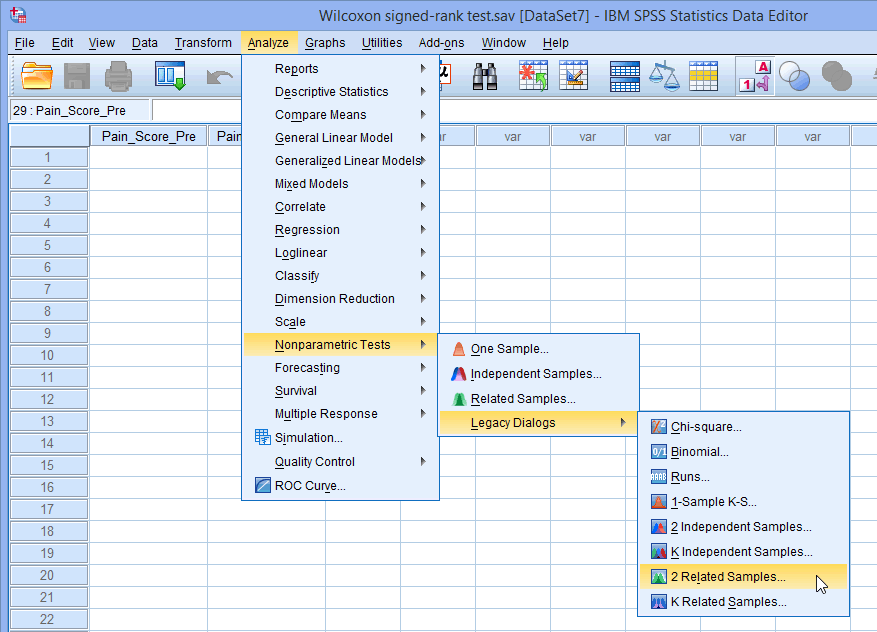
\includegraphics[width=0.7\linewidth]{images/wilcoxon-signed-rank-test-1}
\end{figure}

%Published with written permission from SPSS Statistics, IBM Corporation.

You will be presented with the Two-Related-Samples Tests dialogue box, as shown below:


\subsubsection*{The Wilcoxon Signed-Rank Test Dialog Box}
\begin{figure}
\centering
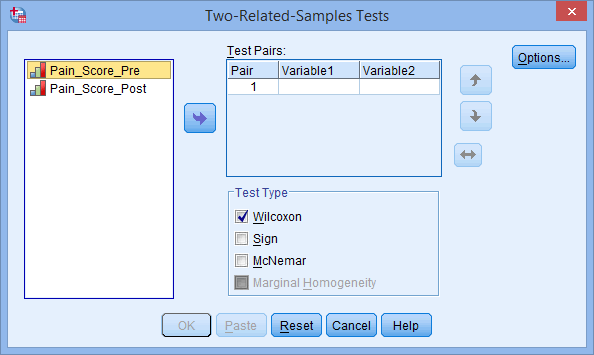
\includegraphics[width=0.7\linewidth]{images/wilcoxon-signed-rank-test-2}
\caption{}
\label{fig:wilcoxon-signed-rank-test-2}
\end{figure}

%Published with written permission from SPSS Statistics, IBM Corporation.
Transfer the variables you are interested in analysing into the Test Pairs: box. In our example, we need to transfer the variables \texttt{Pain\_Score\_Pre} and \texttt{Pain\_Score\_Post}, which represent the Pain Scores before and after the acupuncture intervention, respectively. 

There are two ways to do this. You can either: (1) highlight both variables (use the cursor and hold down the shift key), and then press the SPSS Right Arrow Button button; or (2) drag-and-drop each variable into the boxes. Make sure that the Wilcoxon checkbox is ticked in the –Test Type– area. You will end up with a screen similar to the one below:

\subsection{The Wilcoxon Signed-Rank Test Dialog Box}
\begin{figure}
\centering
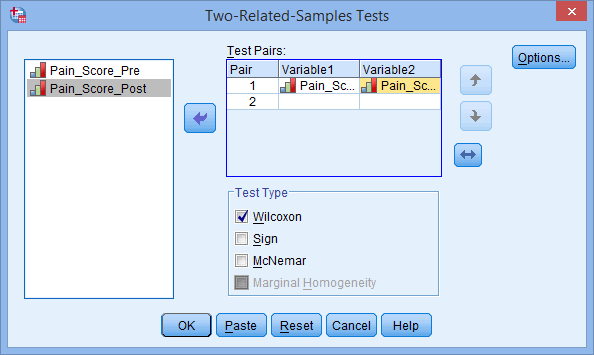
\includegraphics[width=0.7\linewidth]{images/wilcoxon-signed-rank-test-3}
\caption{}
\label{fig:wilcoxon-signed-rank-test-3}
\end{figure}

SPSS Down Arrow Button button shifts the pair of variables you have highlighted down one level.
SPSS Up Arrow Button button shifts the pair of variables you have highlighted up one level.
SPSS Double Arrow Button button shifts the order of the variables within a variable pair.

If you want to generate descriptives or quartiles for your variables, select them by clicking the SPSS Options Button button and ticking the Descriptive and Quartiles checkboxes in the –Statistics– area. Also, you can decide how to deal with missing values. You will end up with a screen similar to the one below:

The Wilcoxon Signed-Rank Test Dialog Box
\begin{figure}
\centering
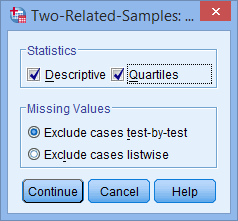
\includegraphics[width=0.7\linewidth]{images/wilcoxon-signed-rank-test-5}
\caption{}
\label{fig:wilcoxon-signed-rank-test-5}
\end{figure}
Click the  button. You will be returned to the Two-Related-Samples Tests dialogue box.

Click the  button.

%======================================================%
\subsection*{SPSS Statistics Output of the Wilcoxon Signed-Rank Test}
SPSS Statistics generates a number of tables in the Output Viewer under the title \textbf{NPar} Tests. In this section, we focus on these three tables to help you understand the results you may obtain when running a Wilcoxon signed-rank test on your data.
\begin{figure}
\centering
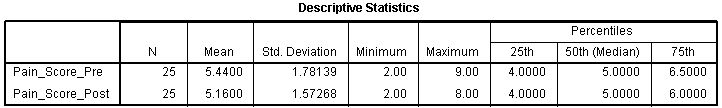
\includegraphics[width=0.7\linewidth]{images/wilcoxon-signed-rank-test-output-1}
\caption{}
\label{fig:wilcoxon-signed-rank-test-output-1}
\end{figure}

\subsection*{Descriptives Table}
The Descriptive Statistics table is where SPSS Statistics has generated descriptive and quartile statistics for your variables if you selected these options. If you did not select these options, this table will not appear in your results. You can use the results from this table to describe the Pain Score scores before and after the acupuncture treatment. As you have used a nonparametric test it is most likely that you should use the quartiles information to describe both your groups.

The Wilcoxon Signed-Rank Test Dialog Box
\begin{figure}
\centering
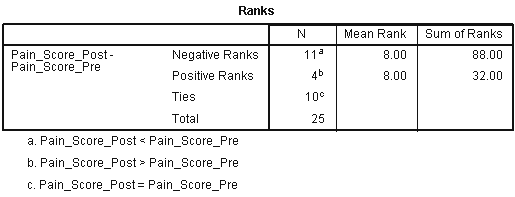
\includegraphics[width=0.7\linewidth]{images/wilcoxon-signed-rank-test-output-2}
\caption{}
\label{fig:wilcoxon-signed-rank-test-output-2}
\end{figure}

\subsubsection*{Ranks Table}
The Ranks table provides some interesting data on the comparison of participants' Before (\texttt{Pre}) and After (\texttt{Post}) Pain Score. We can see from the table's legend that 11 participants had a higher pre-acupuncture treatment Pain Score than after their treatment. However, 4 participants had a higher Pain Score after treatment and 10 participants saw no change in their Pain Score.

The Wilcoxon Signed-Rank Test Dialog Box
Published with written permission from SPSS Statistics, IBM Corporation.

\subsubsection*{Test Statistics Table}
By examining the final Test Statistics table, we can discover whether these changes, due to acupuncture treatment, led overall to a statistically significant difference in Pain Scores. We are looking for the "Asymp. Sig. (2-tailed)" value, which in this case is 0.071. This is the p-value for the test. We report the Wilcoxon signed-ranks test using the Z statistic.

The Wilcoxon Signed-Rank Test Dialog Box
\begin{figure}[h!]
\centering
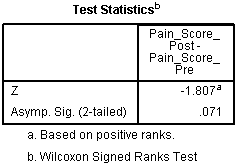
\includegraphics[width=0.7\linewidth]{images/wilcoxon-signed-rank-test-output-3}
\caption{}
\label{fig:wilcoxon-signed-rank-test-output-3}
\end{figure}

Reporting the Output from the Wilcoxon Sign-Rank Test
Based on the results above, we could report the results of the study as follows:

General
A Wilcoxon signed-rank test showed that a 4 week, twice weekly acupuncture treatment course did not elicit a statistically significant change in lower back pain in individuals with existing lower back pain (Z = -1.807, p = 0.071). Indeed, median Pain Score rating was 5.0 both pre- and post-treatment.

In our enhanced Wilcoxon signed-rank test guide, we: (a) show you how to interpret and write up the results of the Wilcoxon signed-rank test irrespective of whether you ran the legacy procedure (as illustrated in this guide) or the newer procedure in SPSS Statistics; (b) provide a more detailed explanation of how to interpret median values and paired differences, as well as negative ranks, positive ranks and ties, and finally, asymptotic p-values; and (c) illustrate how to write up the results from your Wilcoxon signed-rank test procedure if you need to report this in a dissertation/thesis, assignment or research report. We do this using the Harvard and APA styles. 
\end{document}
